\section{Appendix}
\label{appendix}

\subsection{Ablation study}
\label{app:ablation}

In this ablation study, we analyze the impact of key parameters within \Sys. Specifically, we examine the effects of the number of client machines, the number of federated averaging rounds, the number of \gnnshort categorized models, and the anomaly threshold. The effects of these parameters are discussed below:

\PP{Hosts vs Detection Performance} We utilized the \optc dataset for this experiment, randomly selecting a variable number of hosts to participate in training our models through federated learning. The trained global models were then applied to perform threat detection. Figure~\ref{scoresvshosts} presents these results, illustrating that performance improvement is observed up to a certain number of hosts. This plateau is attributed to the \optc dataset's finite set of benign patterns that can be learned. Beyond this threshold, additional hosts do not contribute new information beneficial to the model, thus halting further performance gains and increasing the risk of overfitting. To mitigate this, client machines can monitor the loss of the global model on their local datasets to determine the optimal point to opt out from the learning process.

\begin{figure}[!t]
  \centering
  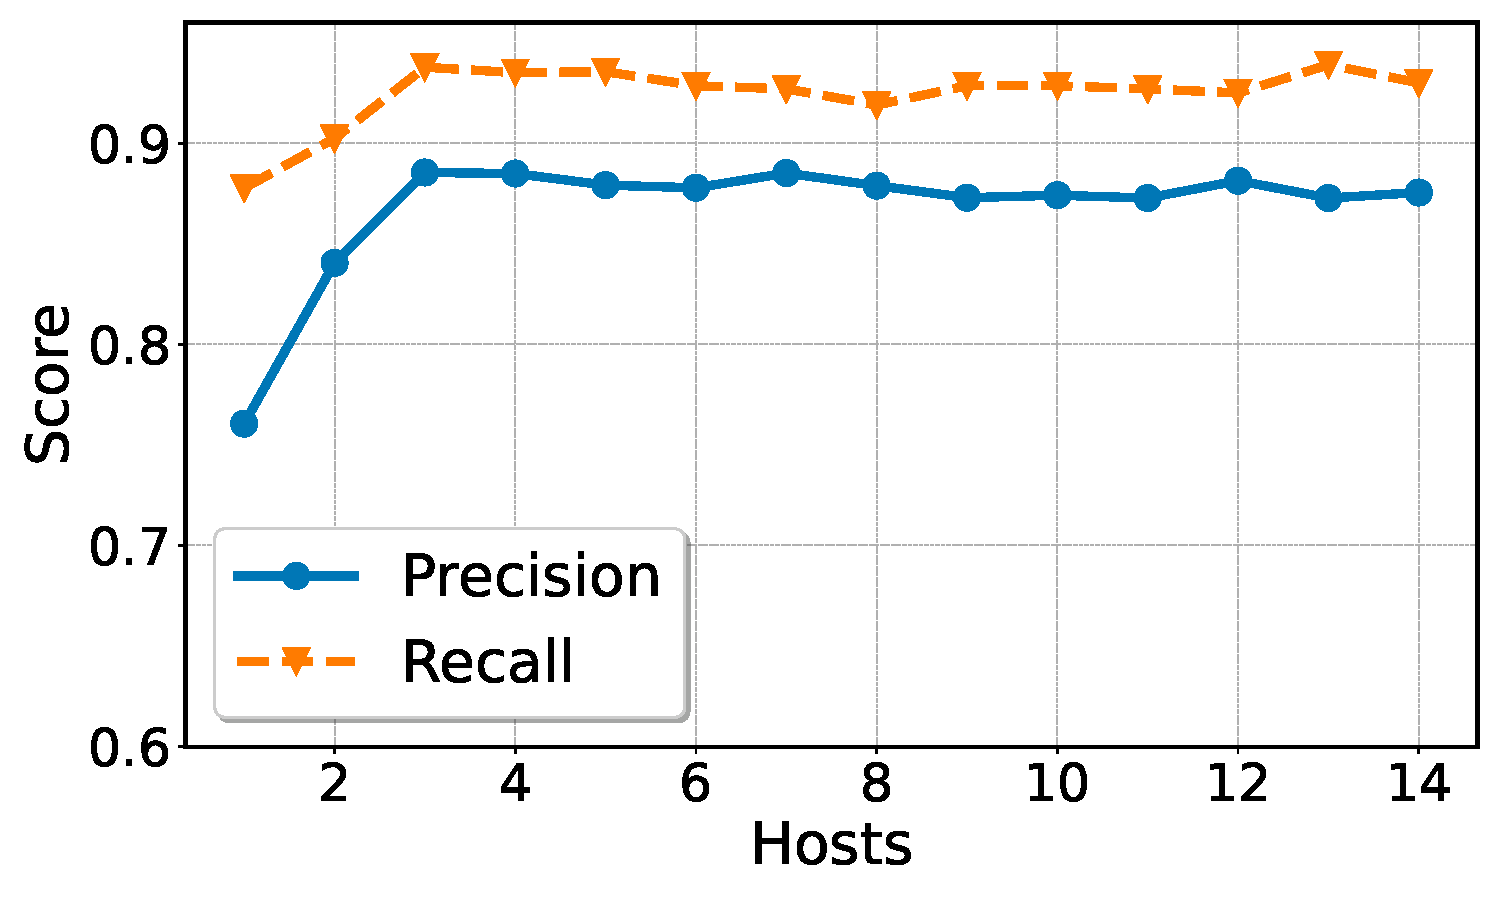
\includegraphics[width=0.3\textwidth]{fig/scoresvshosts.pdf}
  \caption{Effect of number of hosts vs detection metrics using \optc dataset.}
  \label{scoresvshosts}
  \vspace{-2ex}
\end{figure}

\PP{Effect of Federated Averaging Rounds} We employed the \darpa E3 dataset to examine the impact of federated averaging rounds on detection performance. Our methodology involved training the model over a range of federated averaging rounds and subsequently evaluating the model's detection capabilities. The outcomes are depicted in Figure~\ref{roundsvsscore}, which shows that detection performance improves up to a certain number of rounds before declining due to overfitting. Notably, this inflection point is also characterized by a minimal decrease in training loss, suggesting that the model has reached its learning capacity. This observation proves to be a valuable metric for determining the optimal moment to stop training, thereby preventing overfitting and ensuring optimal model performance.

\begin{figure}[!t]
  \centering
  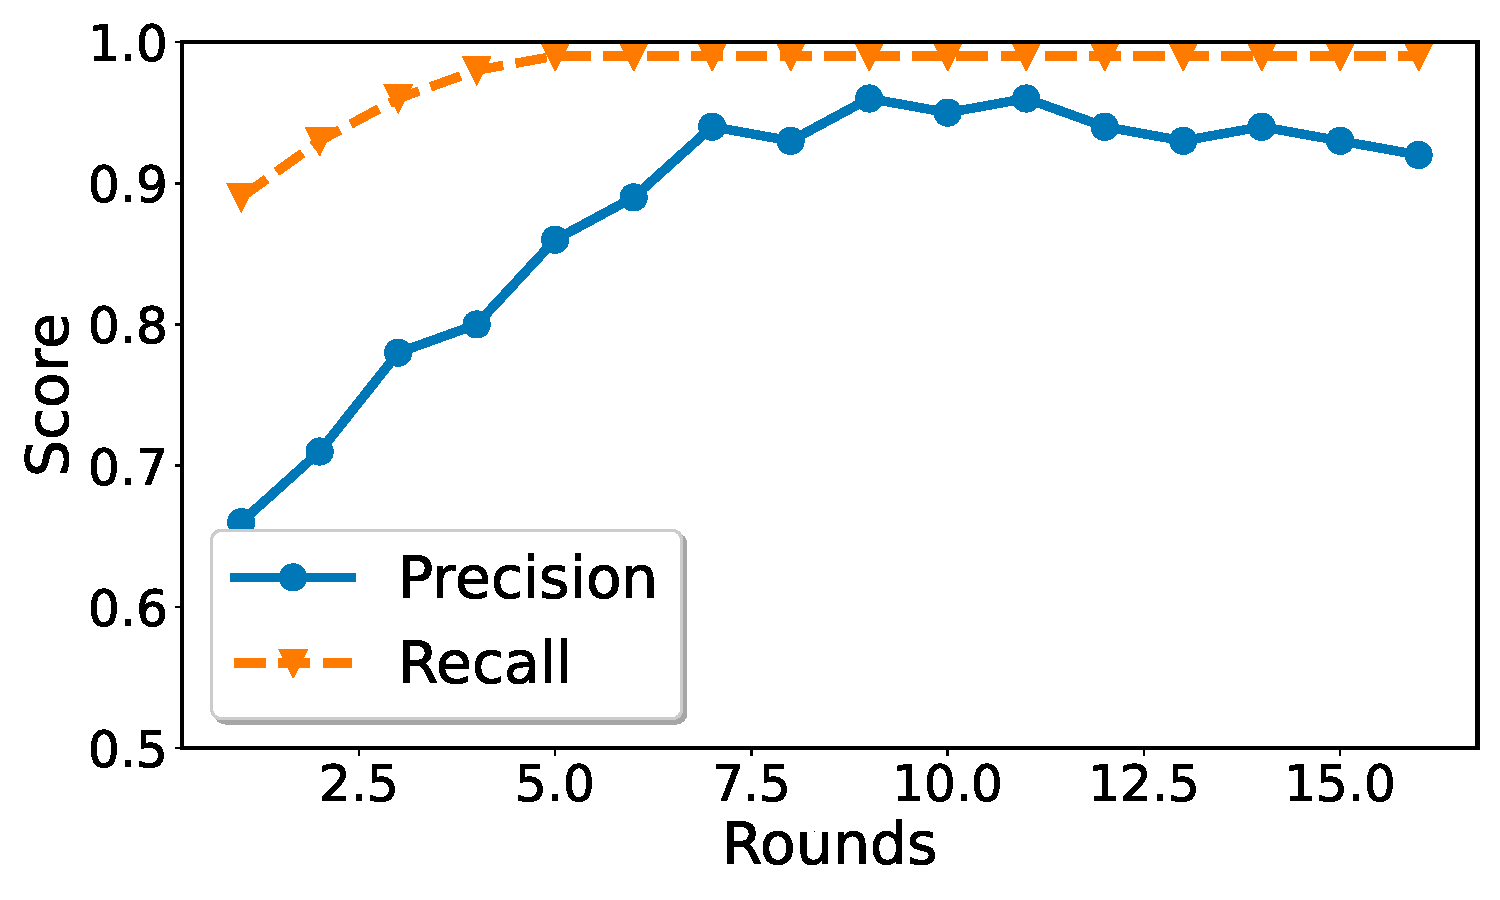
\includegraphics[width=0.3\textwidth]{fig/roundsvsscore.pdf}
  \caption{Federated averaging rounds vs detection performance using E3 dataset. }
  \label{roundsvsscore}
  \vspace{-2ex}
\end{figure}

\PP{Effect number of categories vs Detection} We studied the impact of varying the number of categories ($k$) on the detection performance. Within our system entity-level personalized \gnnshort learning framework, $k$ controls the creation of distinct standardized bins. These bins categorize processes across client machines. Subsequently, we employ an ensemble approach, deploying a separate \gnnshort model for each bin. Thus, the total number of \gnnshort models corresponds to the number of categories. The results depicted in Figure~\ref{catgvsscore} indicate that an increase in $k$ enhances precision while maintaining recall levels. This outcome arises because a single model suffices for achieving high recall by effectively distinguishing between benign and malicious patterns. Nevertheless, a single model falls short in fully generalizing across the diverse benign patterns unique to each client due to the potential blending of individual patterns during the process of federated averaging. Employing a specialized \gnnshort strategy across various categories addresses this challenge by minimizing false alarms.

\begin{figure}[!t]
  \centering
  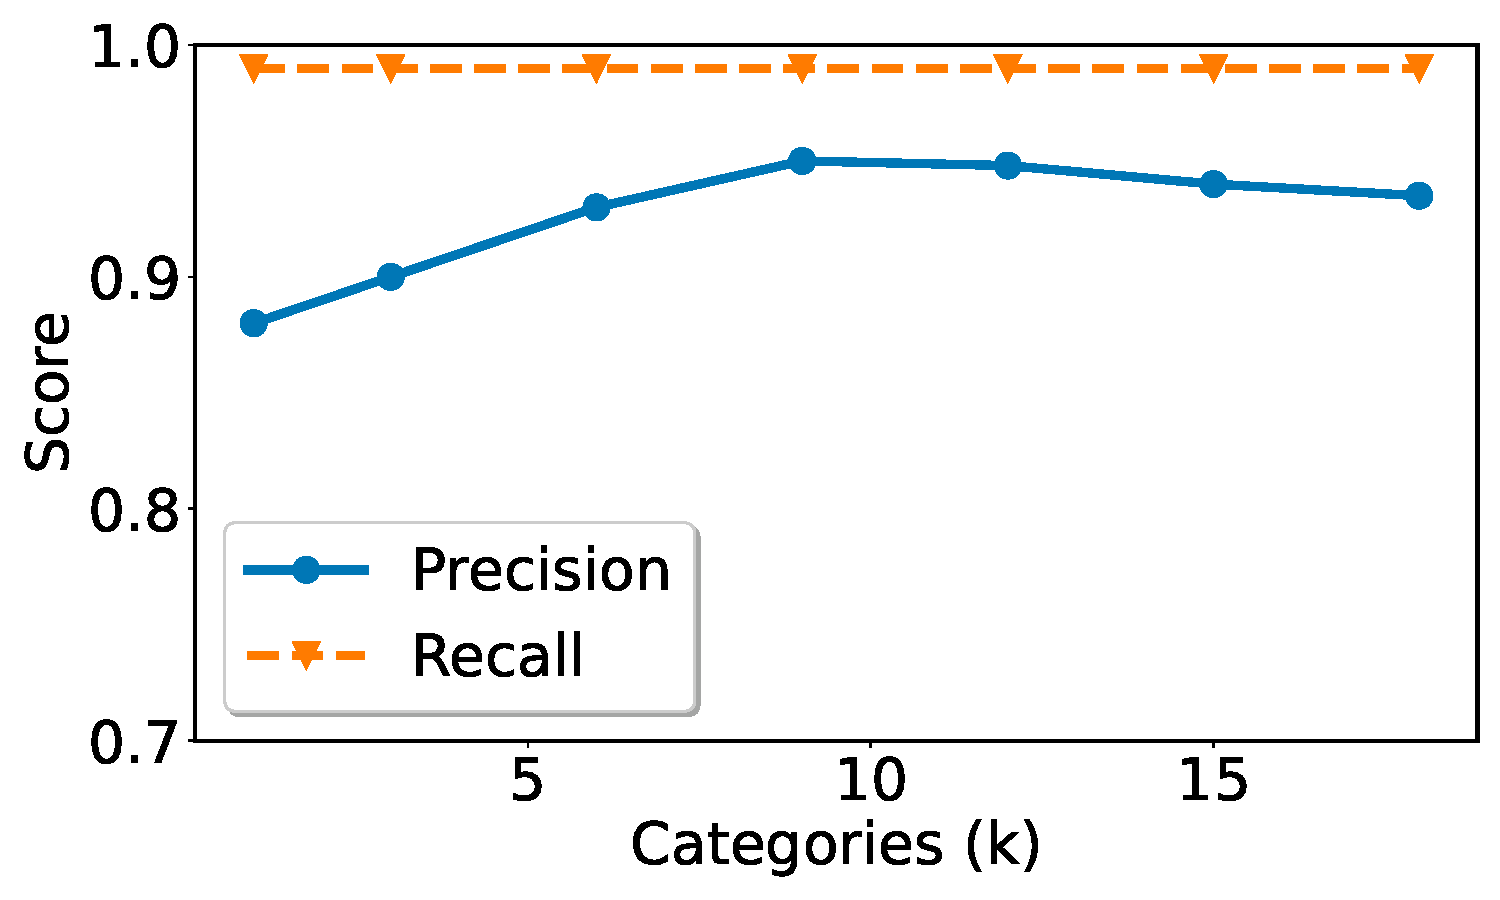
\includegraphics[width=0.3\textwidth]{fig/kvsscore.pdf}
  \caption{Effect of number of categories vs detection performance using E3 dataset.}
  \label{catgvsscore}
  \vspace{-2ex}
\end{figure}

%\subsection{Detection Performance Under Different Methods}

%\wajih{In the Nature's paper they apply different federated learning and GNN approaches to show that the one they propose is best. I remember you tried different FL approaches as well. Also tried if you can replace GNN with something else. In our Flash paper we have something similar where we switched ML methods to show the performance. I would like to see similar experimentation here as well. The idea is to prove that the method that we chose is the best.}

\PP{Effect of number of clients on scalability} \Sys operates in a decentralized manner, ensuring that its scalability post-deployment is independent of the client machines count. After the \fpgl phase concludes, each client runs \Sys locally. However, the number of clients may affect scalability during the training phase, potentially impacting the central and utility servers. The primary function of the central server is to conduct federated averaging on model weights from clients—a straightforward matrix mean operation that requires minimal resources, even with thousands of matrices. Similarly, the utility server's role is to sum and average vectors for overlapping semantic attributes, a task that modern machines are optimized to perform for a large number of samples. Importantly, these operations occur solely during the training phase and do not impact the scalability of the deployed system.

\PP{Anomaly Threshold} This hyperparameter controls the number of alerts generated by \Sys. It determines the trade-off between precision and recall. We use the E5 dataset to investigate the effects of different anomaly thresholds. Figure~\ref{thresh} illustrates the results.

\begin{figure}[!t]
  \centering
  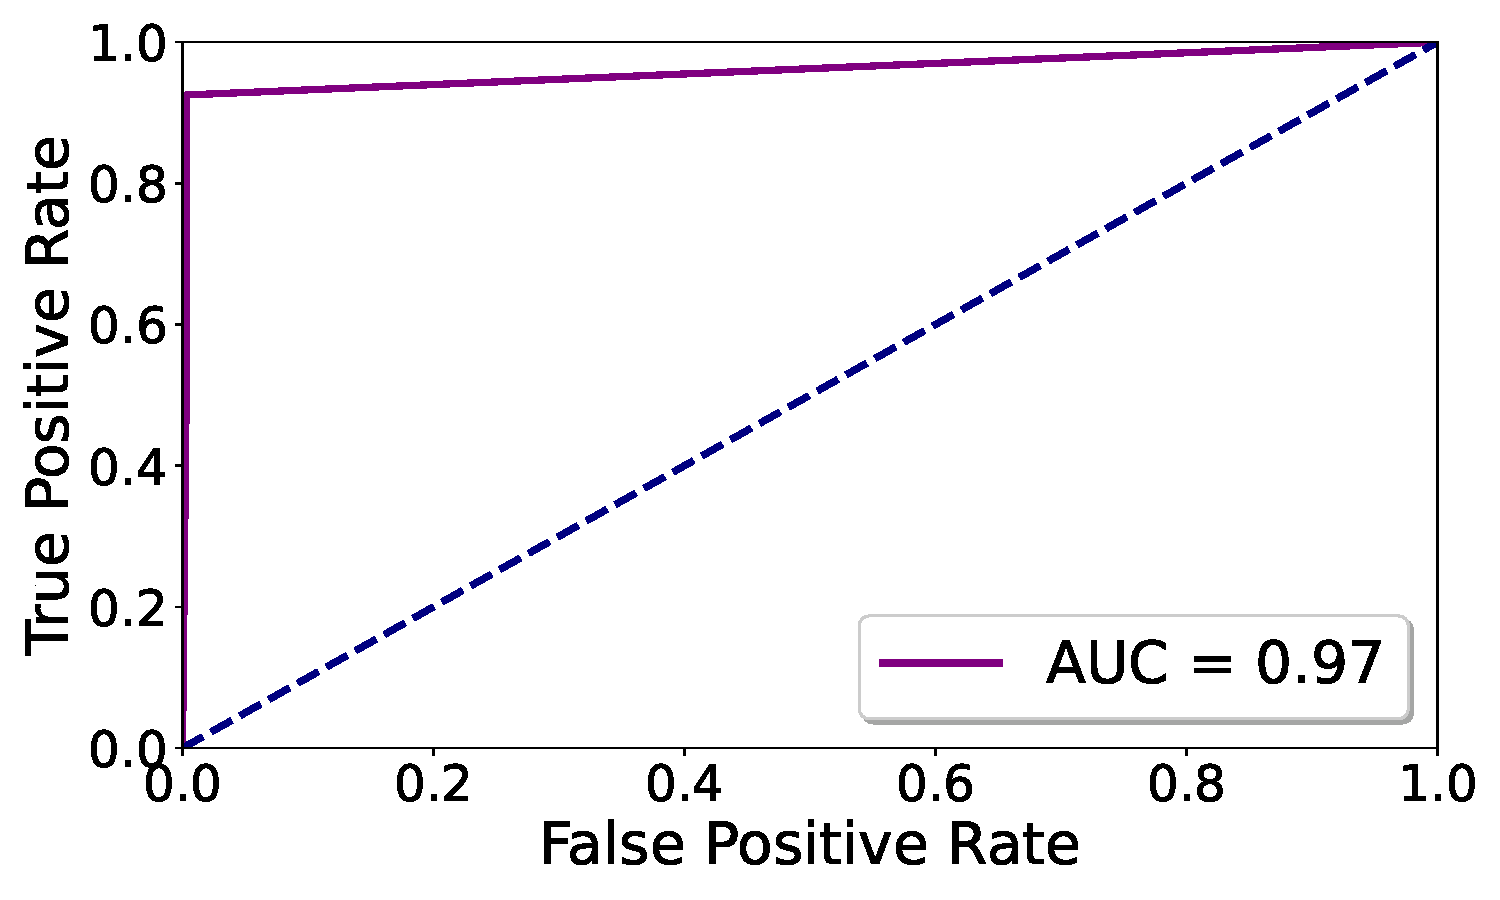
\includegraphics[width=0.3\textwidth]{fig/thresh.pdf}
  \caption{Anomaly threshold effect.}
  \label{thresh}
  \vspace{-2ex}
\end{figure}

% \label{sub:hyper}

% In  federated learning, where data originates from diverse sources such as user machines running various processes, quantifying this diversity becomes crucial for model development. The Shannon Diversity Index (SDI) is a metric adapted from ecology to measure the heterogeneity of datasets. This report elaborates on the application of SDI in federated learning, focusing on comparing the diversity of sub-models in an ensemble approach to a single model scheme.

% \section*{The Shannon Diversity Index (SDI)}

% SDI quantifies a dataset's diversity by considering both the variety of items (richness) and the distribution frequency of each item (evenness). It is given by:

% \[
% H' = -\sum_{i=1}^{R} p_i \ln(p_i)
% \]

% where:
% \begin{itemize}
%     \item $H'$ is the Shannon Diversity Index,
%     \item $R$ denotes the number of unique items,
%     \item $p_i$ represents the proportion of the dataset made up by the $i$th item.
% \end{itemize}

% In federated learning, SDI can reveal the heterogeneity within the data, guiding the strategy for model training and data segmentation.

% \section*{Application of SDI in Federated Learning}

% \subsection*{Scenario Overview}

% A federated learning setup involves analyzing process data from user machines. This scenario examines the diversity of processes, considering the significant overlap among users.

% \subsection*{Example Dataset}

% The dataset features processes like Chrome, Excel, Spotify, and others, from four user machines. Each machine's processes exhibit a 50\% overlap with others, presenting a realistic view of data distribution.

% \subsection*{Process Distribution Across Users}

% \begin{itemize}
%     \item \textbf{User 1}: \{Chrome, Excel, Spotify, Zoom, Slack\}
%     \item \textbf{User 2}: \{Word, PowerPoint, Teams, Slack, Spotify\}
%     \item \textbf{User 3}: \{Chrome, Zoom, Teams, Excel, Word\}
%     \item \textbf{User 4}: \{PowerPoint, Spotify, Slack, Chrome, Word\}
%     \item \textbf{User 5}: \{Chrome, Zoom, Teams\}

% \end{itemize}

% Processes are then randomly divided into three groups.

% \subsection*{Computing SDI for Each Group and single  Scheme}

% SDI calculations are based on the occurrence frequencies of processes, assessing diversity within each group and comparing it to a single  model approach where all processes are considered together.

% \subsubsection*{SDI Results}

% \begin{itemize}
%     \item \textbf{Category 1}: {Chrome, Zoom, and Teams}.
%     \item \textbf{Category 2}: {Word, Excel, and PowerPoint}.
%     \item \textbf{Category 3}: {Spotify and Slack}.
% \end{itemize}

% \subsection*{Analysis and Implications}

% \begin{itemize}
%     \item \textbf{Category 1 SDI}: $H' = 1.08$
%     \item \textbf{Category 2 SDI}: $H' = 1.10$
%     \item \textbf{Category 3 SDI}: $H' = 0.67$
%     \item The single  model, considering all processes together, yielded an SDI of $H' = 2.06$.
% \end{itemize}

% \subsubsection*{Diversity Comparison}

% Compared to the single  model's SDI, each sub-model reflects a specific aspect of the overall diversity but with reduced complexity, suggesting that sub-models focus on more homogeneous subsets of data.

% \subsubsection*{Influence on Client Fairness}

% By dividing the overall task into sub-tasks (sub-models) and assigning them to different subsets of processes (or data features), the influence of clients with large datasets is diversified across multiple models. This can prevent any single client from disproportionately skewing the outcome of the entire federated learning system.

% \subsubsection*{Balanced Representation}

% Each sub-model specializes in a different aspect of the data, potentially leading to a scenario where clients contribute more evenly across the ensemble. Clients with large datasets still contribute significantly, but their impact is more evenly distributed, enhancing fairness.

